\documentclass[11pt,letterpaper]{article}
\usepackage[utf8]{inputenc}

%----- Configuración del estilo del documento------%
\usepackage{epsfig,graphicx}
\usepackage[left=2cm,right=2cm,top=1.8cm,bottom=2.3cm]{geometry}
\usepackage{fancyhdr}
\usepackage{lastpage}
\usepackage{url}
\usepackage{tikz}
\pagestyle{fancy}
\fancyhf{}
\fancyhead[R]{\ifnum\value{page}>1 \textbf{Estadistica Bayesiana}\fi}
\rfoot{\textit{Página \thepage}}
%Encabezado izquierdo: logo
\lfoot{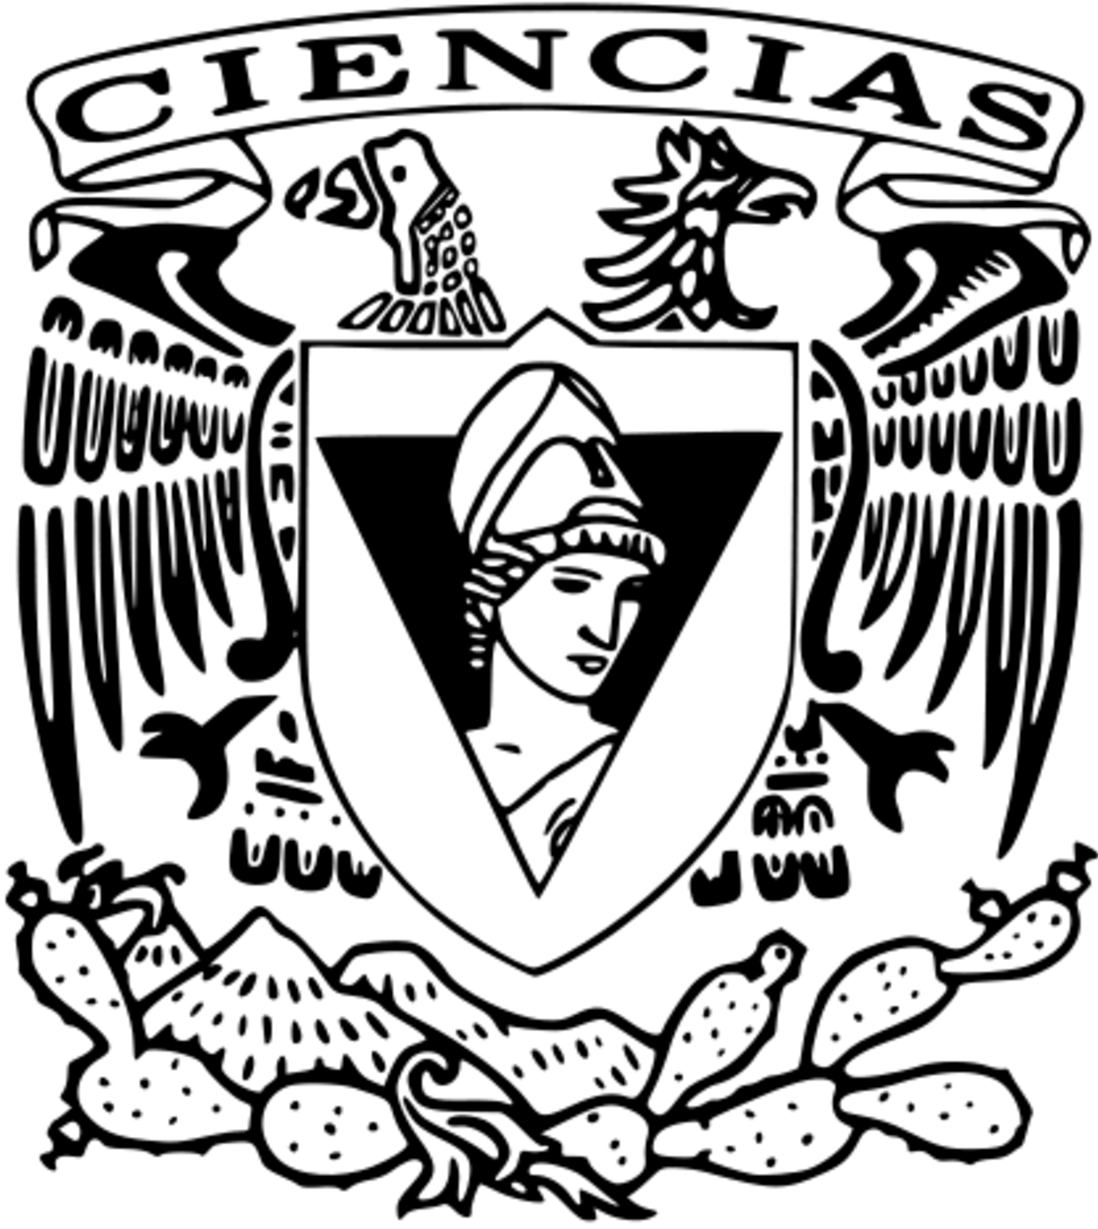
\includegraphics[height=1.0cm]{Logo_FC.png}}
%------ Paquetes matemáticos básicos --------%
\usepackage{amsmath}
\usepackage{amssymb}
\usepackage{amsthm}

\usepackage[spanish]{babel}
\usepackage{graphicx}
\usepackage{hyperref}

\usepackage{tabularx}
\usepackage{xcolor}
\usepackage[table]{xcolor}
\usepackage{colortbl}
\usepackage{array, multirow, multicol, tabularx}
\usepackage{tcolorbox}
\newtheorem{theorem}{Theorem}[section]
\newtheorem{corollary}{Corollary}[theorem]
\newtheorem{lemma}[theorem]{Lemma}

%------si-------%
\definecolor{B}{HTML}{FFFFFF}
\definecolor{G}{HTML}{5e5e5e}
\definecolor{R2}{HTML}{d53d40}
\definecolor{A2}{HTML}{034190}
\definecolor{V2}{HTML}{7faa50}
\newcommand{\R}{\mathbb{R}}
\newcommand{\C}{\mathcal{C}}
\newcommand{\N}{\mathbb{N}}
\newcommand{\Z}{\mathbb{Z}}
\newcommand{\Q}{\mathbb{Q}}
\renewcommand{\theenumi}{\Roman{enumi}}
\renewcommand{\labelenumi}{{\theenumi}.}

\begin{document}
%---Evironment--%
	\makeatletter
        \renewenvironment{proof}[1][\proofname]{\par
            \pushQED{\qed}%
            \normalfont \topsep6\p@\@plus6\p@\relax
            \trivlist
            \item\relax
            {\itshape
            #1\@addpunct{.}}\par\vspace{\baselineskip}\ignorespaces
            }{%
            \popQED\endtrivlist\@endpefalse
            }
        \newenvironment{Solucion}[1][Soluci\'on]{\par
            \pushQED{\qed}%
            \normalfont \topsep6\p@\@plus6\p@\relax
            \trivlist
            \item\relax
            {\itshape
            #1\@addpunct{.}}\par\vspace{\baselineskip}\ignorespaces
            }{%
            \popQED\endtrivlist\@endpefalse
            }
            
    \makeatother

%------ Encabezado -------- %

\begin{center}
    \begin{minipage}{3cm}
    	\begin{center}
    		\includegraphics[height=3.4cm]{logo_unam.png}
    	\end{center}
    \end{minipage}\hfill
    \begin{minipage}{10cm}
    	\begin{center}
    	\textbf{\large Universidad Nacional Autónoma de México}\\[0.1cm]
        \textbf{Facultad de Ciencias}\\[0.1cm]
        \textbf{\'Estadistica Bayesiana}\\[0.1cm]
        Tareita 7 \\[0.1cm]
         El\'ias L\'opez Rivera\\[0.1cm]
        \texttt{ elias.lopezr,@ciencias.unam.mx }\\[0.1cm]
        Fecha:\,\,24/09/2026
    	\end{center}
    \end{minipage}\hfill
    \begin{minipage}{3cm}
    	\begin{center}
    		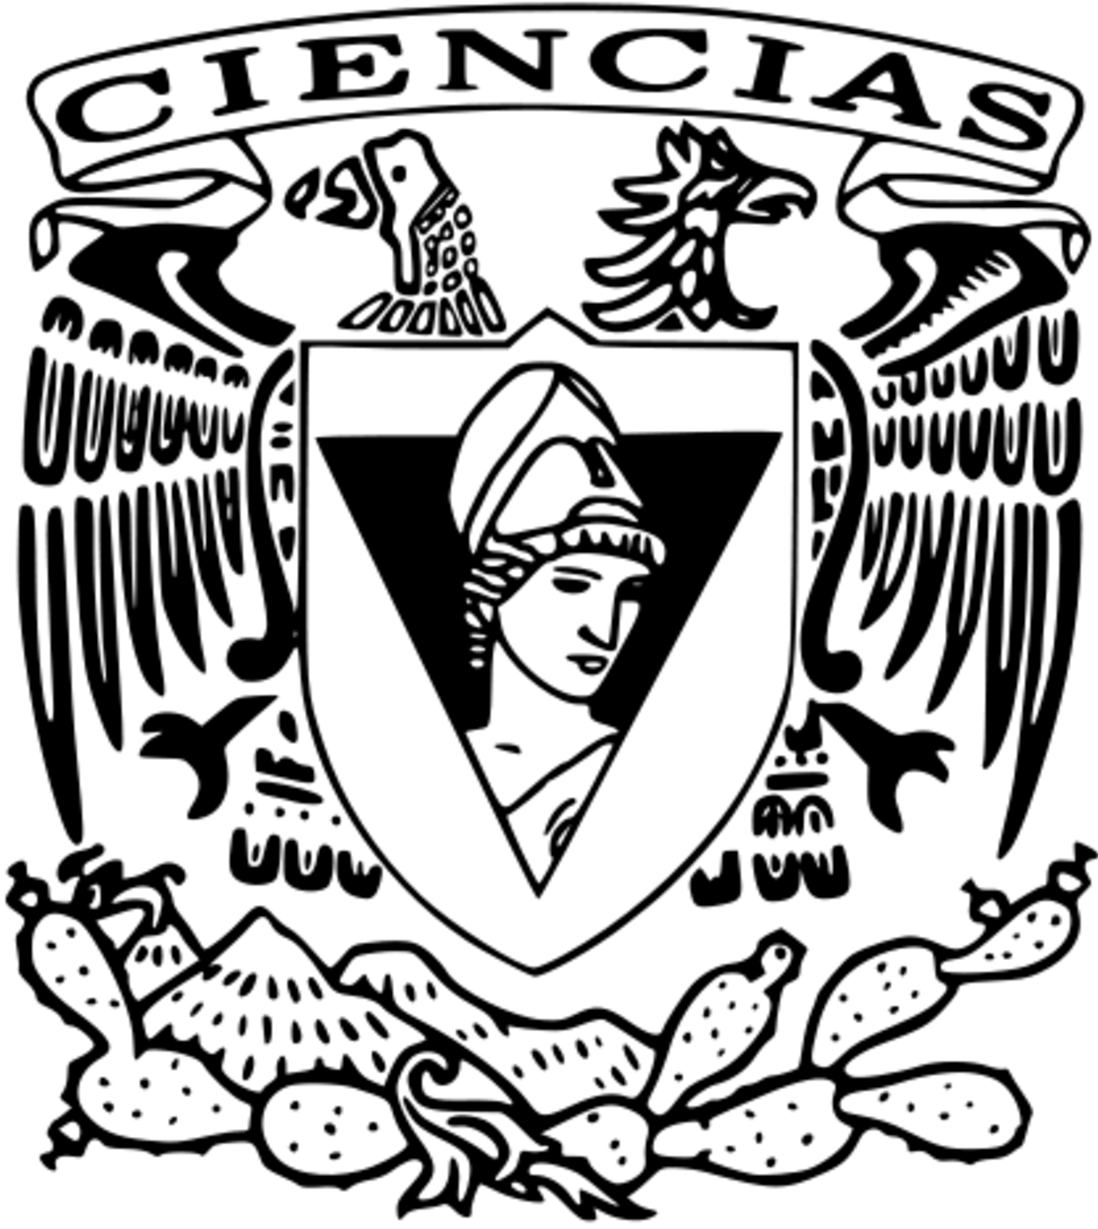
\includegraphics[height=3.4cm]{Logo_FC.png}
    	\end{center}
    \end{minipage}
\end{center}
\rule{17cm}{0.1mm}
%------ Fin de encabezado -------- %
\begin{tcolorbox}[
	title = \textcolor{black}{\textcolor{white}{Problema 1}},]
\textit{Sean variables aleatorias intercambibales que condicionadas al parametro $\theta=(h,w)$ se distribuyen $x\sim N(x|w,h)$ 
considerando que la distribuci\'on conjunta inicial de $\theta$ es una normal-Gamma $(h,w)\sim N(h|\mu,\tau h)Ga(h|\alpha,\beta)$ mostrar
que la marginal de $w$ es una $t$ de student }
\end{tcolorbox}
\begin{proof}
    Tenmeos que $(w|h)\sim N(w|\mu,\tau h)$ y por tanto $h\sim Ga(h|\alpha,\beta)$, por tanto usando proba total tenemos que:\,\\
    \begin{align*}
        p(w)&=\int_{\theta}p(w|h)p(h)dh=\frac{\beta^{\alpha}\sqrt{\tau}}{\sqrt{2\pi }\,\Gamma(\alpha)}\int_{\theta}e^{-\frac{h\tau}{2}(w-\mu)^2}h^{\alpha-1}\sqrt{h}e^{-\beta h}\,dh\,\\
        \,\\
        &=\frac{\beta^{\alpha}\,\sqrt{\tau}}{\sqrt{2\pi}\Gamma(\alpha)}\int_{\theta} e^{-h(\frac{\tau (w-\mu)^2}{2}+\beta)}h^{\alpha+\frac{1}{2}-1}\,dh
    \end{align*}
    Reconocemos inmediatamente el kernel de una $Gamma$ para $\bar{\alpha}=\alpha+\frac{1}{2}$ y $\bar{\beta}=\frac{\tau}{2}(w-\mu)^2+\beta$ por tanto:\,\\
    \begin{align*}
        p(w)&=\frac{\beta^{\alpha}\sqrt{\tau}\,\Gamma(\alpha+\frac{1}{2})}{\sqrt{2\pi}\Gamma(\alpha)}\frac{1}{\left(\frac{\tau}{2}(w-\mu)^2+\beta\right)^{\alpha+\frac{1}{2}}}=\frac{\beta^{\alpha}\sqrt{\tau}\,\Gamma(\alpha+\frac{1}{2})}{\sqrt{2\pi}\Gamma(\alpha)}(\beta)^{-\alpha-\frac{1}{2}}\left[\frac{\tau\,(w-\mu)^2}{2\,\beta}+1\right]^{-\alpha-\frac{1}{2}}\,\\
        \,\\
        &=\frac{\Gamma(\alpha+\frac{1}{2})}{\Gamma(\alpha)}\sqrt{\frac{\tau}{2\pi\,\beta}}\left[\frac{\tau\,(w-\mu)^2}{2\,\beta}+1\right]^{-\alpha-\frac{1}{2}}=stu\left(w|2\alpha,\mu,\frac{\tau\alpha}{2\beta}\right)
    \end{align*}
\end{proof}
\end{document}